\chapter{Diseño}
\section{Casos de Uso}
\subsection{Diagramas de Casos de Uso}
A través de los diagramas de casos de uso se representan los diferentes servicios que la aplicación ofrece.

La Figura \ref{fig:Diagrama-de-Casos-de-Uso-de-Administrador} presenta el diagrama de casos de uso para la gestión de administradores.

\begin{figure}[ht] 
\centering
\caption{Diagrama de Casos de Uso de Administrador}
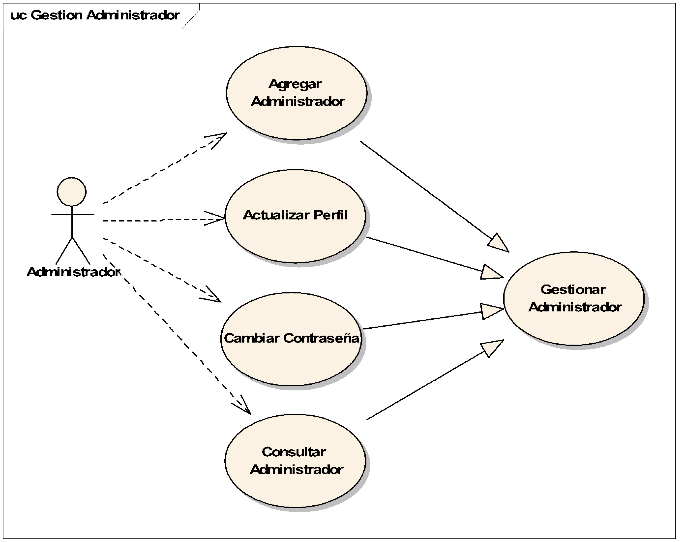
\includegraphics[width=0.5\textwidth]{img/cuAdministrador.png}
\label{fig:Diagrama-de-Casos-de-Uso-de-Administrador}  
\end{figure} 

La Figura \ref{fig:Diagrama-de-Casos-de-Uso-de-Pago} presenta el diagrama de casos de uso para la gestión de pago.

\begin{figure}[ht] 
\centering
\caption{Diagrama de Casos de Uso de Pago}
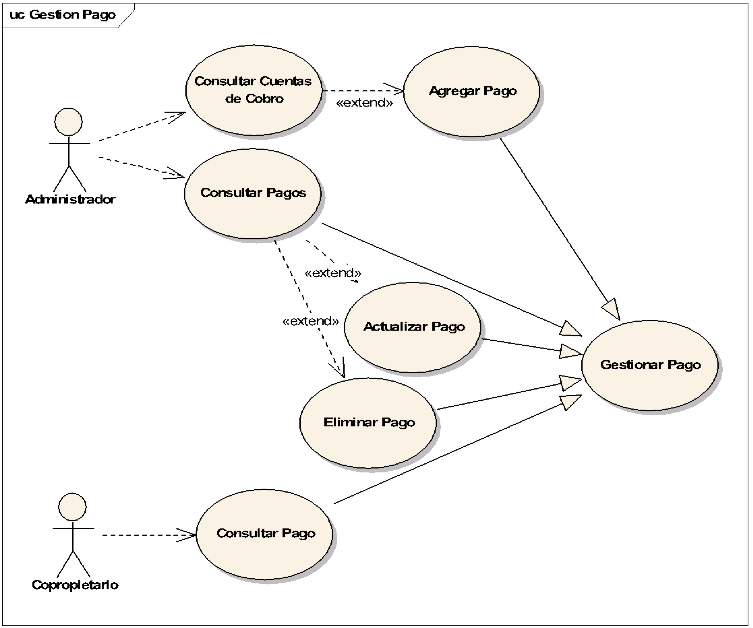
\includegraphics[width=0.6\textwidth]{img/cuPago.png}
\label{fig:Diagrama-de-Casos-de-Uso-de-Pago}  
\end{figure} 

\subsection{Documentación de Casos de Uso}
La documentación de casos de uso describe las características de cada uno de ellos así como el flujo de eventos de interacción entre el actor que participa y el sistema. La Tabla \ref{table:Documentacion-de-Casos-de-Uso} describe los casos de uso del sistema.

\begin{center}
\begin{longtable}{p{2.5cm} p{12cm}}
\caption{Documentación de Caso de Uso}
\label{table:Documentacion-de-Casos-de-Uso}
\\ \hline \hline
\textbf{ID} & \textbf{CU 01} \\ \hline
\textbf{Nombre} & \textbf{Registrar Usuario} \\ \hline
\textbf{Descripción} & El usuario se registra en el sistema ingresando los datos solicitados \\ \hline
\textbf{Actor} & Usuario \\ \hline 
\textbf{Precondicion} & El usuario no debe existir en el sistema \\ \hline
\textbf{Poscondicion} & El usuario se crea en el sistema \\ \hline 
\textbf{Eventos} & 
\begin{minipage}[t]{1\linewidth}
\begin{tabular}{|p{5.5cm}|p{5.5cm}|} \hline
\textbf{Actor} & \textbf{Sistema} \\ \hline
1. Ingresa los datos solicitados &  \\ \hline
& 2. Valida la información \\ \hline
& 3. Ingresa la información \\ \hline
& 4. Genera un mensaje de confirmación \\ \hline
\end{tabular}
\end{minipage} 
\\ \hline
\textbf{Excepción} & Ninguno \\ \hline
\textbf{Autor} & Hector Florez \\ \hline
\textbf{Fecha} & Agosto de 2014 \\ \hline
\hline \\ \hline \hline

\textbf{ID} & \textbf{CU 02} \\ \hline
\textbf{Nombre} & \textbf{Realizar Pago} \\ \hline
\textbf{Descripción} & El usuario paga los productos que se encuentran en el carro de compras \\ \hline
\textbf{Actor} & Usuario \\ \hline 
\textbf{Precondicion} & El usuario debe estar autenticado en el sistema. El carro de compras debe tener al menos un producto \\ \hline
\textbf{Poscondicion} & Los productos del carro de compras quedan en estado \textit{Pagado} \\ \hline 
\textbf{Eventos} & 
\begin{minipage}[t]{1\linewidth}
\begin{tabular}{|p{5.5cm}|p{5.5cm}|} \hline
\textbf{Actor} & \textbf{Sistema} \\ \hline
1. Ingresa al servicio de pagos &  \\ \hline
2. Ingresa información de pago & \\ \hline
& 3. Valida información de pago \\ \hline
& 4. Cambia estado de los productos del carro de compras \\ \hline
& 5. Envía correo electrónico con los detalles del pago \\ \hline
& 6. Genera un mensaje de confirmación \\ \hline
\end{tabular}
\end{minipage} 
\\ \hline
\textbf{Excepción} & Si la validación de la información de pago no es exitosa, el pago no se lleva a cabo, los productos no cambian de estado y se envía un correo electrónico reportando el fallo de validación \\ \hline
\textbf{Autor} & Hector Florez \\ \hline
\textbf{Fecha} & Agosto de 2014 \\ \hline
\hline \\ \hline \hline

\textbf{ID} & \textbf{CU 03} \\ \hline
\textbf{Nombre} & \textbf{Habilitar Usuario} \\ \hline
\textbf{Descripción} & El administrador habilita un usuario registrado \\ \hline
\textbf{Actor} & Administrador \\ \hline 
\textbf{Precondicion} & El usuario debe existir en el sistema. El administrador debes estar autenticado \\ \hline
\textbf{Poscondicion} & El usuario es habilitado \\ \hline 
\textbf{Eventos} & 
\begin{minipage}[t]{1\linewidth}
\begin{tabular}{|p{5.5cm}|p{5.5cm}|} \hline
\textbf{Actor} & \textbf{Sistema} \\ \hline
1. Consulta usuario &  \\ \hline
& 2. Retorna información \\ \hline
3. Habilita usuario &  \\ \hline
& 4. Cambia estado del usuario \\ \hline
\end{tabular}
\end{minipage} 
\\ \hline
\textbf{Excepción} & Si la consulta no arroja resultados, el sistema no presenta la opción de habilitar usuario \\ \hline
\textbf{Autor} & Hector Florez \\ \hline
\textbf{Fecha} & Agosto de 2014 \\ \hline
\end{longtable}
\end{center}

\section{Diagrama de Clases}
Con base en los casos de uso y su documentación se crea el diagrama de clases que se presenta en la Figura \ref{fig:Diagrama-de-Clases}. El diagrama de clases cuenta con las siguientes clases:
\begin{itemize}
    \item \texttt{Usuario}. Esta clase representa...
    \item \texttt{Administrador} ...
\end{itemize}

\begin{figure}[ht] 
\centering
\caption{Diagrama de Clases}
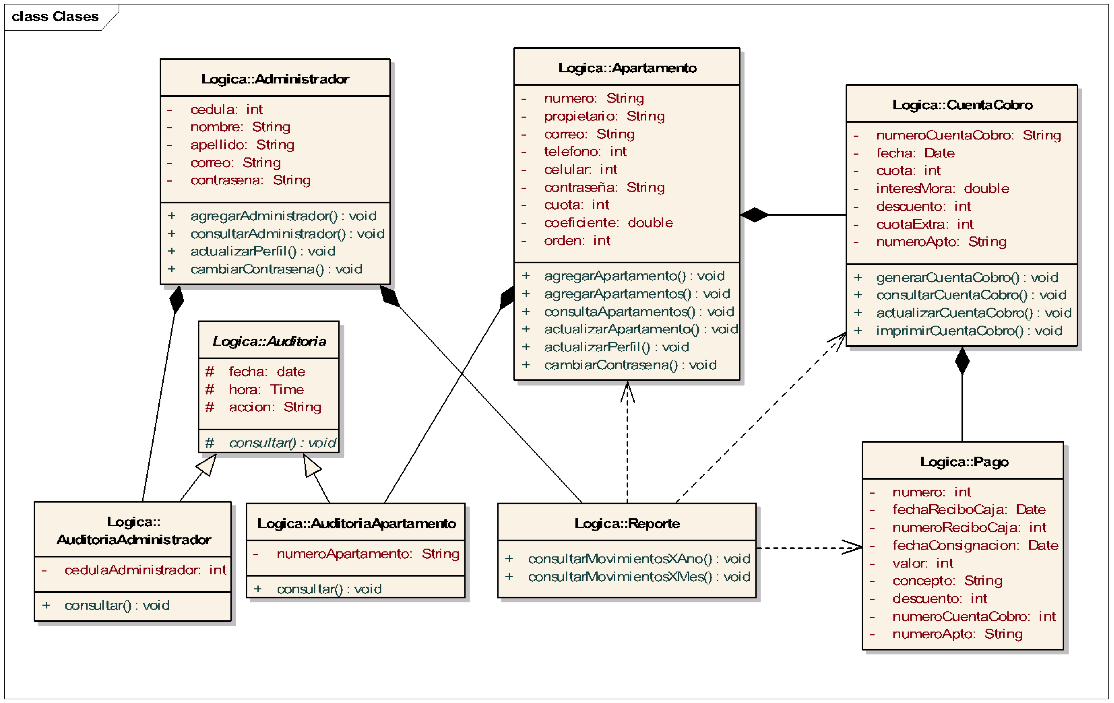
\includegraphics[width=0.8\textwidth]{img/diagramaClases.png}
\label{fig:Diagrama-de-Clases}  
\end{figure} 

\section{Diagramas de Secuencia}

\section{Diagramas de Componentes}

\section{Diagramas de Despliegue}

